\documentclass[a4paper,10pt,oneside]{book}

\usepackage[utf8]{inputenc}
\usepackage{float}
%Uma das dificuldades para os usuários do Latex é o posicionamento das figuras, já que ele tenta fazer isso de forma otimizada e automática. Se o usuário quizer forçar as figuras existem duas possibilidades:(1) Definir o posicionamento em: (h) aqui, (t) topo, (b) base, ou na (p) página. O uso do ! siginifica para forçar a solicitação do usuário. a ordem [htb] indica a preferencia que o latex vai re-arranjar as figuras.%(2%) Muitas vezes o usuário não quer otimizar o espaço do texto. Ou seja que posicionar a figura em determinado lugar mesmo que um pedaço da págian fique em branco. Neste caso o indicado é usar o pacote: float e o posicionamento H.%
\usepackage{hyperref}
\usepackage{graphicx}
\usepackage{textcomp}
\usepackage{gensymb}
\usepackage[table,xcdraw]{xcolor}
\usepackage{listings}
\usepackage{cmap}
\usepackage[T1]{fontenc}
\usepackage{verbatim}
\usepackage[table,xcdraw]{xcolor}
\usepackage{longtable}
\usepackage{multirow}

\usepackage[brazil]{minitoc}
\mtcsettitle{minitoc}{Lista de Exemplos}
\newcommand{\filterminitoc}[1]{#1}
\renewcommand{\thesection}{\csname filterminitoc \endcsname{\arabic{chapter}.}\arabic{section}}
\newcommand{\minitocsection}{\begingroup\renewcommand{\filterminitoc}[1]{}\minitoc\endgroup}

% Configurando layout para mostrar codigos C++
\usepackage{listings}
% Definindo novas cores
\usepackage{color}

\usepackage{geometry}
	\geometry{
	a4paper,
	total={170mm,257mm},
	left=40mm,
	right=30mm,
	top=40mm,
	bottom=30mm,
 }

\definecolor{mygreen}{rgb}{0,0.6,0}
\definecolor{mygray}{rgb}{0.5,0.5,0.5}
\definecolor{black}{rgb}{0.3,0.3,0.3}
\definecolor{gray}{rgb}{0.9,0.9,1}
\definecolor{mymauve}{rgb}{0.58,0,0.82}
\lstset{ %
  backgroundcolor=\color{white},  
  basicstyle=\ttfamily\small,            
  breakatwhitespace=false,         
  breaklines=true,                 
  captionpos=b,                    
  commentstyle=\color{mygreen},  
  deletekeywords={...},            
  escapeinside={\%*}{*)},  
  extendedchars=true,    
  %frame=single,	                  
  keepspaces=true,                 
  keywordstyle=\color{blue},       
  language=Octave,,                 
  otherkeywords={*,...},          
  numbers=left,                   
  numbersep=5pt,                   
  numberstyle=\ttfamily\small\color{mygray},
  rulecolor=\color{black},         
  showspaces=false,                
  showstringspaces=false,          
  showtabs=false,                  
  stepnumber=2,                    
  stringstyle=\color{mymauve},  
  tabsize=2,	                   
  title=\lstname,
}


\lstdefinestyle{citacao}{ %
  backgroundcolor=\color{white},   % choose the background color; you must add \usepackage{color} or \usepackage{xcolor}
  basicstyle=\ttfamily,        % the size of the fonts that are used for the code
  breakatwhitespace=false,         % sets if automatic breaks should only happen at whitespace
  breakautoindent=true,
  %breaklines=true,                 % sets automatic line breaking
  columns=fixed,			% don't add spaces between characters
  commentstyle=\color{mygreen},    % comment style
  deletekeywords={...},            % if you want to delete keywords from the given language
  escapeinside={\%*}{*)},          % if you want to add LaTeX within your code
  extendedchars=true,              % lets you use non-ASCII characters; for 8-bits encodings only, does not work with UTF-8
  frame=simple,	                   % adds a frame around the code
  keepspaces=true,                 % keeps spaces in text, useful for keeping indentation of code (possibly needs columns=flexible)
  keywordstyle= \color{blue}\bf,       % keyword style
  language=C,                 % the language of the code
  otherkeywords={},           % if you want to add more keywords to the set
  numbers=left,                    % where to put the line-numbers; possible values are (none, left, right)
  numbersep=5pt,                   % how far the line-numbers are from the code
  numberstyle=\normalfont\color{mygray}, % the style that is used for the line-numbers
  rulecolor=\color{black},         % if not set, the frame-color may be changed on line-breaks within not-black text (e.g. comments (green here))
  showspaces=false,                % show spaces everywhere adding particular underscores; it overrides 'showstringspaces'
  showstringspaces=false,          % underline spaces within strings only
  showtabs=false,                  % show tabs within strings adding particular underscores
  stepnumber=1,                    % the step between two line-numbers. If it's 1, each line will be numbered
  stringstyle=\color{mymauve},     % string literal style
  tabsize=4,	                   % sets default tabsize to 2 spaces
  title=\lstname                   % show the filename of files included with \lstinputlisting; also try caption instead of title
}

\lstdefinestyle{funcao}{ %
  backgroundcolor=\color{white},   % choose the background color; you must add \usepackage{color} or \usepackage{xcolor}
  basicstyle=\ttfamily,        % the size of the fonts that are used for the code
  breakatwhitespace=false,         % sets if automatic breaks should only happen at whitespace
  breakautoindent=true,
  %breaklines=true,                 % sets automatic line breaking
  columns=fixed,			% don't add spaces between characters
  commentstyle=\color{mygreen},    % comment style
  deletekeywords={...},            % if you want to delete keywords from the given language
  escapeinside={\%*}{*)},          % if you want to add LaTeX within your code
  extendedchars=true,              % lets you use non-ASCII characters; for 8-bits encodings only, does not work with UTF-8
  frame=trBL,	                   % adds a frame around the code
  frameround=T,
  rulesep=1pt,
  framesep=5pt,
  rulesepcolor=\color{gray},
  framexleftmargin=-20pt,
  xleftmargin=-20pt,
  xrightmargin=0pt,
  keepspaces=true,                 % keeps spaces in text, useful for keeping indentation of code (possibly needs columns=flexible)
  keywordstyle=\normalcolor\normalfont\normalsize,       % keyword style
  language=C,                 % the language of the code
  otherkeywords={},           % if you want to add more keywords to the set
  numbers=none,                    % where to put the line-numbers; possible values are (none, left, right)
  rulecolor=\color{black},         % if not set, the frame-color may be changed on line-breaks within not-black text (e.g. comments (green here))
  showspaces=false,                % show spaces everywhere adding particular underscores; it overrides 'showstringspaces'
  showstringspaces=false,          % underline spaces within strings only
  showtabs=false,                  % show tabs within strings adding particular underscores
  stringstyle=\color{mymauve},     % string literal style
  tabsize=4,	                   % sets default tabsize to 2 spaces
  title=\lstname                   % show the filename of files included with \lstinputlisting; also try caption instead of title
}




\title{Desenvolvimento em microcontroladores baseados em processadores ARM Cortex-M4 com TivaWare}
\author{
        Leandro Fabian Junior\\
        \and
        Callebe Soares Barbosa\\
        \and
        Orientador: Gustavo Weber Denardin
}
\date{2016}


%renomeia o titulo dos tipos figure
\renewcommand{\figurename}{Figura}
%renomeia o titulo dos tipos Table
\renewcommand{\tablename}{Tabela} 
\renewcommand{\lstlistingname}{Código} 
\renewcommand{\chaptername}{Capítulo}
\renewcommand{\contentsname}{Índice}
\renewcommand{\bibname}{Referências}
\renewcommand{\listfigurename}{Lista de Figuras}
\renewcommand{\listtablename}{Lista de Tabelas}

\graphicspath{{figuras/}{fig_site/}}

\newcommand{\ttbu}[1]{\texttt{\textbf{\underline{#1}}}}

\usepackage{ifthen}

\newcommand{\forloop}[5][1]%
{%
\setcounter{#2}{#3}%
\ifthenelse{#4}%
	{%
	#5%
	\addtocounter{#2}{#1}%
	\forloop[#1]{#2}{\value{#2}}{#4}{#5}%
	}%
% Else
	{%
	}%
}%

% How to use:    \forloop[step]{counter}{initial_value}{conditional}{code_block}
% 
% For example:
% 
% \newcounter{ct}
% \forloop{ct}{1}{\value{ct} < 5}%
% {%
% \arabic{ct}
% }



\begin{document}
%\maketitle

\begin{titlepage}
	\newgeometry{left=3cm, bottom=3cm, right=3cm, top=3cm}
	\centering
% 	\begin{minipage}{1\textwidth}
% 	\begin{multicols}{2}	
% 	\begin{minipage}{.5\textwidth}
% 		\begin{flushright}
% 			\begin{center}
% 			\includegraphics[width=.9\textwidth]{logo_utfpr.png}\par\vspace{1cm}
% 			\end{center}
% 		\end{flushright}
% 	\end{minipage}
% 	\begin{minipage}{.5\textwidth}
% 		\begin{flushleft}
% 			\scshape \LARGE Universidade Tecnológica Federal do Paraná\par
% 		\end{flushleft}
% 	\end{minipage}
% 	\end{multicols}
% 	\end{minipage}
%\includegraphics[width=.3\textwidth]{logo_utfpr.png}\par\vspace{10pt}
\rule{\textwidth}{1pt}
{\scshape \LARGE Universidade Tecnológica Federal do Paraná\par\vspace{5pt} \Large Campus Pato Branco}
	\rule{\textwidth}{1pt}
	\vfill
	{\huge\bfseries Desenvolvimento em microcontroladores baseados em processadores ARM Cortex-M4\par}
	\vfill
	\begin{minipage}{\textwidth}
		\centering
		\Large\itshape Leandro Fabian Junior\par
		\Large\itshape Callebe Soares Barbosa\par
	\end{minipage}
	\vspace{2cm}
	
	{orientado por\par
	\Large\itshape Gustavo Weber Denardin}

	\vfill

% Bottom of the page
	{\large2016\par}
	\newpage
	\pagenumbering{gobble}
 \vfill
  \begin{center}
   {\scshape \LARGE Universidade Tecnológica Federal do Paraná\par\vspace{5pt} \Large Campus Pato Branco} \\[2.5cm]

   \begin{minipage}{\textwidth}
		\centering
		\Large\itshape Leandro Fabian Junior\par
		\Large\itshape Callebe Soares Barbosa\par
	\end{minipage}
	\vspace{1cm}
	
	{orientado por\par
	\Large\itshape Gustavo Weber Denardin}
	\vfill

   {\huge\bfseries Desenvolvimento em microcontroladores baseados em processadores ARM Cortex-M4\par}
   \vfill

   \hspace{.45\textwidth} %posiciona a minipage
   \begin{minipage}{.5\textwidth}
   \large Recurso Educacional Aberto produzido com o fomento do Programa de Bolsas para o Desenvolvimento de Recursos Educacionais Abertos (PIBEA) por meio do Programa de Bolsas de Fomento às Ações de Graduação da UTFPR
  \end{minipage}
  \vfill
  \hspace{11cm}
  %\includegraphics[width=3cm]{Cc-by-nc-sa_icon.png}
	
\vspace{2cm}

{\large2016\par}
\end{center}
\end{titlepage} 

\pagenumbering{arabic}
\setcounter{page}{2}
\listoffigures
\listoftables

\dominitoc
\nomtcrule
\tableofcontents

\chapter{Introdução}
O material aqui contido busca iniciar o leitor no desenvolvimento em plataformas baseadas em processadores com arquitetura ARM.

Inicialmente, o texto introduz alguns conceitos sobre a arquitetura ARM, em especial as Cortex-M3 e M4. São discutidos seus registradores padrão e seus modos de operação. Após isso, são abordadas as características das plataformas específicas utilizadas nos exemplos deste material. Os \emph{hardwares} utilizados aqui, são o kit de 
avaliação Tiva\textsuperscript{TM} C Series TM4C1294NCPDT, e o MSP432P401R. Ambos da empresa Texas Instruments.

Logo após, são introduzidos os padrões utilizados neste material: a biblioteca TivaWare e o padrão CMSIS. Ainda, são mostrados métodos de utilizá-los a partir da IDE da Texas Instruments, o Code Composer Studio.

Os capítulos centrais abordam algumas características do TM4C1294NCPDT, e ainda, como são implementadas através da TivaWare. São abordados a maioria dos periféricos principais, sendo que cada capítulo aborda um deles em especial.

Ao final, são apresentados exemplos práticos de implementação dos principais periféricos. Tanto utilizando a TivaWare, para o TM4C1294NCPDT, quanto utilizando a CMSIS, para o MSP432P401R.


\chapter{Conhecendo o Processador ARM}
\subsection{Características ARM}

Com o objetivo de desenvolver aplicações em processadores ARM se faz necessário aqui uma breve apresentação das características desta arquitetura. 

O termo ARM (Advanced RISC Machine) se refere a uma arquitetura que usa de forma avançada o conceito conhecido como RISC (Reduced Instruction Set Computer). Este conceito é uma linha de arquitetura que favorece um conjunto simples e pequeno de instruções que levam aproximadamente a mesma quantidade de tempo para serem executadas, permitindo que estes processadores tenham menos transístores do que aqueles projetados na arquitetura convencional. Logo essa abordagem reduz a liberação de calor, o consumo de energia e a quantidade de componentes em um processador.

A arquitetura dos processadores usados aqui, o Cortex-M3 e Cortex-M4, são ambos as implementações da arquitetura ARMv7-M. Existem diferentes tipos de arquitetura ARM para diferentes tipos de processadores, que ainda podem variar conforme são atualizadas ao longo dos anos. Os detalhes da arquitetura ARMv7-M estão documentados no Manual de Referência da Arquitetura  ARMv7-M, disponível no site da  \href{http://infocenter.arm.com/help/index.jsp}{ARM Limited}.

O Cortex-M3 e Cortex-M4 são essencialmente idênticos em seus aspectos construtivos, de modo que o diagrama de blocos da figura \ref{DiagramaDeBlocosARM}  apresenta uma visão  geral interna adequada tanto do processador Cortex –M4 quanto -M3.

\begin{figure}[H]
	\centering
	\includegraphics[scale=0.9]{DiagramaDeBlocosARM}
	\caption{Diagrama de Blocos - Processador Cortex-M3 e Cortex-M4 \cite{DATASHEET_TIVA}}
	\label{DiagramaDeBlocosARM}
\end{figure}

Na figura \ref{DiagramaDeBlocosARM} notamos a presença de elementos no processador como:  o controlador de vetores de interrupção, NVIC (\emph{Nested Vectored Interrupt Controller}); o controlador de acionamento de interrupção, WIC (\emph{Wakeup Interrupt Controller}); o temporizador SysTick; a unidade de proteção de memória, MPU (\emph{Memory Protection Unit}); e uma unidade de ponto flutuante presente apenas no Cortex –M4. Existe ainda um sistema de debug dentro do processador para realizar depuração de software e um sistema interno de barramentos para transferência de dados entre o núcleo do processador, o sistema de debug e o MPU. 

Os processadores da família Cortex M são de 32 bits, podendo também trabalhar com dados de 8 bits e 16 bits de forma bastante eficiente. Já os processadores Cortex-M3  e Cortex-M4, mesmo sendo da família Cortex M, podem realizar uma série de operações envolvendo dados de 64 bits. Estas operações podem ser realizadas através de um \emph{piperline} de três estágios com uma arquitetura de barramento do tipo \emph{Harvard} permitindo instruções simultâneas de busca e acesso de dados.

Uma das grandes vantagens dos processadores Cortex M é seu baixo consumo de energia. Em especial os processadores Cortex M3 e Cotex M4 podem executar instruções com taxa de $200 mA/MHz$ com alimentação de $1,8 V$. Estes processadores possuem modos de suspensão que tornam possíveis desativar dispositivos de \emph{Clock} para economizar energia, e um \emph{hardware} adicional para despertar o processador dos modos de suspensão.

Devemos salientar aqui que estamos sempre nos referindo a apenas aos processadores, e que este é uma parte constituinte do microcontrolador. De modo que os demais componentes da placa são desenvolvidos pelos diferentes fabricantes. Assim existem vários tipos de microcontroladores com diferentes características de periféricos e recursos, porém a arquitetura empregada nos processadores é a mesma.


\subsection{Modos de operação ARM Cortex-M4}

O processador Cortex-M4 possui dois estados de operação, como mostrado na figura \ref{fig:modosDeOperacao}, \emph{debug state} e \emph{Thumb state}. O \emph{debug state} ocorre quando o processador é interrompido, por exemplo ao atingir um \emph{breakpoint}, então a execução de instrução é interrompida. Já o \emph{Thumb state} ocorre quando o código do programa está sendo executado. Diferente de outros processadores ARM, o Cortex-M não suporta instruções ARM.

\begin{figure}[H]
	\centering
	\includegraphics[scale=0.9]{modosDeOperacaoCortex-M4}
	\caption{Modos de Operação \cite{DATASHEET_TIVA}}
	\label{fig:modosDeOperacao}
\end{figure}

No \emph{Thumb state} ainda existem dois modos de operação, que dizem respeito ao nível de privilégio no acesso ao processador. Ao executar uma rotina de tratamento de interrupção o processador entra em um nível de acesso privilegiado, caracterizando o \emph{handler mode}. Durante a execução de uma aplicação normal o processador pode estar tanto em nível de acesso privilegiado quanto em nível menor, sendo chamado de \emph{thread mode}. Isso é controlado por um registrador específico. 

A aplicação pode alterar seu nível de acesso durante o \emph{thread mode}, para um nível menos privilegiado. Porém, para aumentar seu nível de acesso deve haver um mecanismo de exceção/interrupção por parte do processador.  Tais mecanismos de controle de nível de acesso garantem uma maior robustez para o sistema, controlando o acesso à regiões críticas de memória.

\subsubsection{Registradores internos}

Para um controle melhor e um processamento de dados maior o Cortex-M4 possui registradores internos ao processador agrupados em um conjunto chamado de \emph{banco de registradores}. Cada instrução enviada ao processador especifica a operação a ser executada, os registradores fonte e se necessário os registradores de destino. A arquitetura ARM é baseada no modelo conhecido como \emph{load/store}, ou seja, para processar um conteúdo que esteja na memória é preciso carregá-lo para um registrador interno e então processá-lo. Se necessário, é preciso armazená-lo de volta na memória.

\begin{figure}[H]
	\centering
	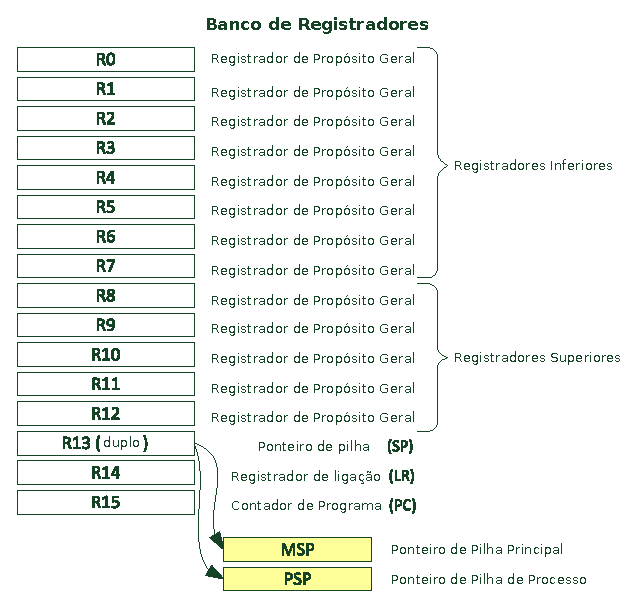
\includegraphics[scale=0.9]{bancoRegistradores}
	\caption{Banco de registradores internos \cite{DATASHEET_TIVA}}
	\label{fig:bancoRegistradores}
\end{figure}

O banco de registradores do Cortex-M4 possui 16 registradores de 32 bits, como mostrado na Figura \ref{fig:bancoRegistradores}. Cada registrador possui seu propósito, como detalhado a seguir:

\begin{description}
\item[R0 - R12: Registradores de Propósito Geral]\hfill \\
Devido ao número limitado no conjunto de instruções, muitas das de 16 bits somente acessam os registradores de R0 à R7, chamados de \emph{registradores inferiores}. De R8 à R9, os \emph{registradores altos}, podem ser usados com as instruções de 32 de bits e alguns com instruções 16 de bits. Os valores iniciais desses registradores são indefinidos.

\item[R13: Ponteiro de Pilha (\emph{Stack Pointer}, SP)]\hfill \\
Usado para acessar a pilha de memória. Fisicamente há dois ponteiros de pilha, o principal (\emph{Main Stack Pointer}, MSP) e o de processo (\emph{Process Stack Pointer}, PSP)). O MSP é o ponteiro padrão, é selecionado após um \emph{reset} do sistema ou quando o processador está em modo de exceção (Handler Mode). Seu valor inicial é o primeiro da memória na sequência de \emph{reset}. Já o PSP é usado durante o Thread Mode, quando as tarefas da aplicação estão rodando, seu valor inicial é desconhecido.

Somente um dos ponteiros de pilha é visível durante a aplicação e os dois bits menos significativos de ambos são sempre nulos. Em aplicações que não fazem uso de um sistema operacional somente o MSP é usado.

\item[R14: Registrador de Ligação (\emph{Link Register}, LR)]\hfill \\
Esse registrador armazena automaticamente o ponto em que uma rotina chama uma sub-rotina. Assim, ao fim da execução dessa sub-rotina, esse valor é carregado para o Contador de Programa e a execução continua de onde tinha anteriormente parado.

Se uma sub-rotina chamar outra sub-rotina, o valor nesse registrador será substituído e o ponto de retorno antigo se perderá, portanto é preciso que esse último valor seja salvo na pilha de memória.

Durante uma rotina de tratamento de exceção, o valor de LR é também sobrescrito mas por um valor de retorno de exceção, usado para disparar o retorno da exceção ao fim da rotina de tratamento.

\item[R15: Contador de Programa (\emph{Program Counter, PC})]\hfill \\
Marca o próximo endereço que deve ser executado na aplicação. Quando este registrador é lido, automaticamente seu valor decrementa de 4 (32 bits), apontando para o próximo endereço da execução. Já quando é feito uma operação de escrita, o programa pula para a posição apontada e passa a executar a aplicação a partir deste novo ponto.

O bit menos significativo do PC indica o tipo de instrução que está sendo executada, '0' para ARM e '1' para Thumb. Portanto no Cortex-M4, tal bit deve ser sempre '1' pois não são suportadas instruções ARM. Este fato deve ser lembrado quando é feita uma operação de escrita sobre o registrador.

\end{description}





\chapter{Conhecendo a plataforma de trabalho}
O hardware utilizado aqui será o  TIVA \texttrademark ~~ TM4C1294NCPDT, um kit de desenvolvimento da empresa Texas Instruments que possui um microcontrolador baseado no processador ARM Cortex-M4. A tabela \ref{tab:CaracteristicasMicro} traz suas principais características.

%% TABELA DE CARACTERISTICAS BASICAS %%%%%%%%%%

% \begin{table}[!h]
% \centering

\begin{longtable}{|l|l|}

\hline
\cellcolor[HTML]{343434} \color[HTML]{FFFFFF} Características & \cellcolor[HTML]{343434} \color[HTML]{FFFFFF} Descrição \\
\hline
Núcleo & ARM Cortex-M4F\\
\hline
Performance & Operação até 120-MHz; 150 DMIPS \\
& (Dhrystone MIPS) de performance \\
\hline
Memória Flash & 1024 KB  \\
\hline
SRAM & 256 KB single-cycle System SRAM \\
\hline
EEPROM & 6KB  \\
\hline
ROM & ROM interna carregada com biblioteca  \\
 & TivaWare™  C Series \\
\hline
Interface de Periféricos Externos (EPI)  & Interface dedicada de 8-/16-/32-   \\ 
 &  bits dedicados a periféricos e memoria\\
\hline
 Verificação de Redundância & Função Hash de 16-/32- bits,  que suporta  \\
  Cíclica (CRC)   & quatro formas de CRC \\
\hline
\begin{comment}
 Função de Adulteração & Suporte para quatro entradas de  \\
 & adulteração e resposta de evento de  \\
 & adulteração configurável configurável  \\
\hline
\end{comment}
Universal Asynchronous  & 8 módulos UARTs \\
Receivers/Transmitter (UART) & \\
\hline
Quad Synchronous Serial & Quatro módulos de SSI com Bi- , Quad-\\
Interface (QSSI) &  e suporte avançado de SSI\\
\hline
Inter-Integrated Circuit ($I^{2}C$) & 10 módulos $I^{2}C$ com 4 velocidades \\
 & de transmissão\\
\hline
Controller Area Network (CAN) & 2 controladores CAN 2.0 A/B \\
\hline
Ethernet MAC & 10/100 Ethernet MAC \\
\hline
Ethernet PHY & PHY com IEEE 1588 PTP \\
\hline
Universal Serial Bus (USB) & USB 2.0 OTG/Host/Device  \\ 
& com ULPI interface e suporte a Link   \\
& Power Management (LPM) \\
\hline
Micro Acesso Direto à Memória ($\mu DMA$) & Controlador ARM$\copyright$ PrimeCell$\copyright$  \\
& 32-channel configurável  $\mu DMA$ \\
\hline
General-Purpose Timer (GPTM) & 8 blocos 16/32-bit GPTM \\
\hline
Watchdog Timer (WDT) & 2 Watchdog Timers \\
\hline
Hibernation Module (HIB) & Low-power battery-backed \\
 & Hibernation module \\
\hline
General-Purpose Input/Output (GPIO) & 15 physical GPIO blocks \\
\hline
Pulse Width Modulator (PWM) & 1 modulo PWM , com 4 geradores PWM  \\
 & e um  registador de controle,\\
 &  com um total de 8  saídas PWM.\\
\hline
Quadrature Encoder Interface (QEI) & Um modulo QEI \\
\hline
Analog-to-Digital Converter (ADC) & 2 modulos ADC de 12-bit\\
 & taxa de 2 milhões de amostras/segundo\\
\hline
Controlador Comparador Analógico & Três comparadores analógicos \\
& independentes \\
\hline
Comparador Digital & 16 comparadores digitais \\
\hline
JTAG e Serial Wire Debug (SWD) & 1 modulo JTAG  com ARM SWD\\
& integrado \\
\hline
Encapsulamento & 128-pin TQFP \\
\hline
Temperatura de Operação & $-40 \degree C$ até $105 \degree C$ \\
\hline
\caption{Características Básicas - TM4C1294NCPDT \cite{DATASHEET_TIVA}}
\label{tab:CaracteristicasMicro}
\end{longtable}
% \end{table}

%%%%%%%%%%%%%%%%%%%%%%%%%%%%%%%%%%%%%%%%%%%%%%%%%%%%%%%


O TM4C1294NCPDT possui dois barramentos. Um desses é responsável pela conexão padrão entre o núcleo de processamento e os periféricos, o \emph{Advanced Peripheral Bus} (APB). Já o outro, o \emph{Advanced High-Performance Bus} (AHB), é um barramento especial que pode ser requisitado da maioria dos periféricos e, possui uma resposta muito mais rápida por ser exclusivo. O esquema dos barramentos é mostrado no diagrama de blocos da figura \ref{fig:DiagramaBlocosTiva}.


\begin{figure}[H]
\centering
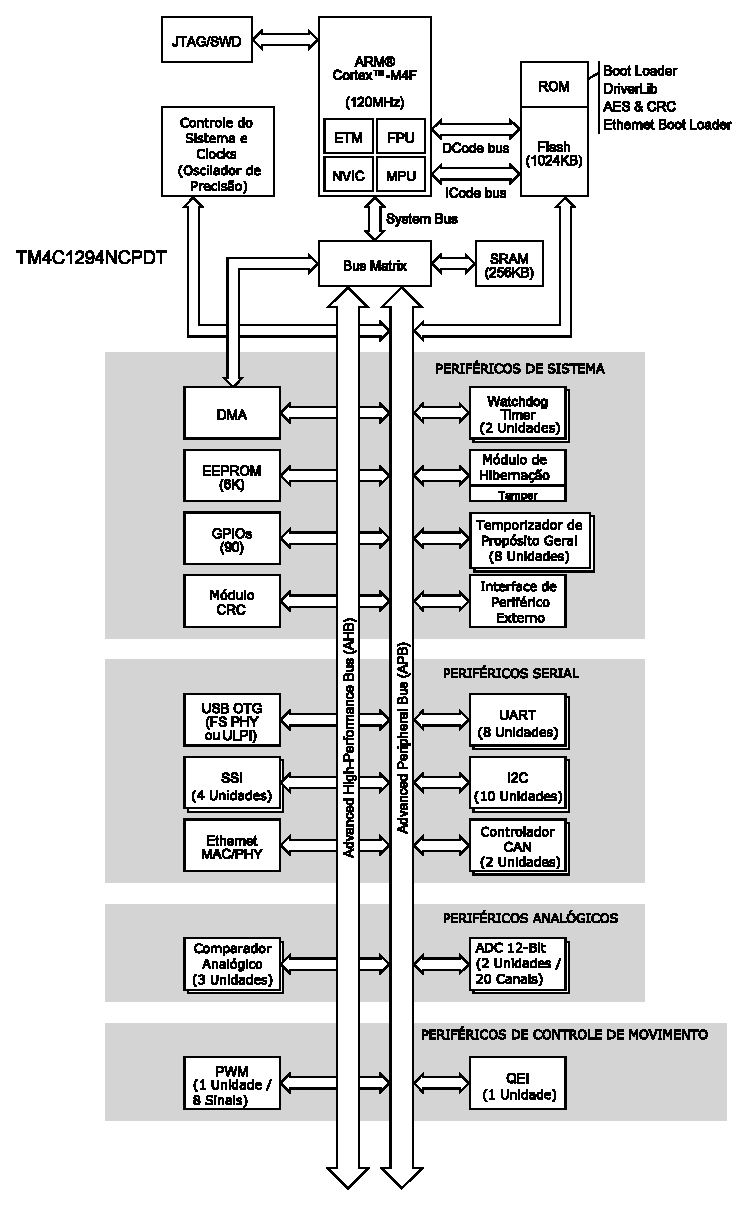
\includegraphics[width=0.8\textwidth] {DiagramaBlocosTiva.eps}
    \caption{Diagrama de Blocos - TM4C1294NCPDT \cite{DATASHEET_TIVA}}
    \label{fig:DiagramaBlocosTiva}
\end{figure}

%%%%%%%%%%%%%%%%%%%%%%%%%%%%%%%%%%%%%%%%%%%%%%%%%%%%%%%

\chapter{Iniciando um projeto no Code Composer}
\input{src/iniciandoUmProjetoNoCodeComposer.tex}

\chapter{Biblioteca TivaWare}
Para facilitar a programação do microcontrolador será feito o uso da biblioteca TivaWare fornecida pela Texas Instruments. Tal ferramenta facilita o controle do processador e acesso aos periféricos disponíveis. A TivaWare pode ser obtida no site da empresa gratuitamente.

O site disponibiliza somente a versão para o sistema Windows, que vem em formato executável, sendo preciso apenas dar um clique duplo sobre o arquivo e seguir os passos da instalação. Já para sistemas não derivados do \emph{MS-DOS}, basta abrir este mesmo executável baixado com um aplicativo de descompactação de arquivos e copiar o conteúdo para um diretório qualquer desejado.

A estrutura do TivaWare é composta basicamente de dois diretórios \cite{TivaWare}:

\begin{description}
	\item [driverlib/] Contém o código fonte para os drivers do dispositivo
	\item [inc/] Contém os arquivos de cabeçalho que são usados pelos drivers para acessar os registradores do microcontrolador
\end{description}

Os outros arquivos contidos no pacote do TivaWare são extras que facilitam alguns usos do microcontrolador. Como o diretório \emph{'examples/'} que contém códigos prontos para utilização em alguns dos microcontroladores e periféricos suportados, o \emph{'utils/'} com algumas implementações frequentes e a biblioteca \emph{'usblib/'} que implementa uma comunicação usb com portes para vários tipos de arquivos.


\section{Incluindo a TivaWare  ao projeto}

Para a utilização da TivaWare nos projetos que serão apresentados é preciso que as aplicações desenvolvidas tenham acesso à tais bibliotecas. Tal comunicação pode ser feita de dois tipos: \emph{linkando} ou copiando a biblioteca para o diretório do código fonte ou adicionando o diretório da biblioteca nos comandos de compilação.

\subsection{Bibliotecas junto ao código fonte}

Este método pode ser feito de dois modos, copiando as bibliotecas para o diretório do código fonte da aplicação, ou \emph{linkando}-as a este diretório.

É importante notar que se os arquivos de código fonte forem portados para outra máquina, somente serão compilados se as bibliotecas estiverem disponíveis nesta. Portanto, sempre que houver memória disponível, é aconselhável que se copie as bibliotecas usadas na aplicação para junto de seu diretório.

Para copiar as bibliotecas é possível apenas copiar as pastas para o diretório do projeto que este será atualizado automaticamente ou ainda arrastar e soltar o diretório ou arquivo da biblioteca sobre o projeto na barra lateral \emph{Project Explorer} no Code Composer que será aberta uma janela intermediária como na figura \ref{fig:janelaCopiarLinkar}.

Selecionando \textbf{'Copy files and folders'} os arquivos serão copiados para o diretório do projeto escolhido. Já as duas outras opções criarão somente um \emph{link} do arquivo no diretório especificado na caixa de seleção \textbf{'Create link location relative to'}, deste modo o compilador verá os arquivos como se eles estivessem neste diretório, porém existe apenas o caminho para alcançá-los. Se acaso eles forem movidos haverá erros de compilação.

\begin{figure}[H]
\centering
\includegraphics[width=0.8\textwidth] {janelaCopiarLinkar.png}
    \caption{Janela de importação de arquivos}
    \label{fig:janelaCopiarLinkar}
\end{figure}

\subsection{Inclusão de caminho na compilação}

Um outro modo de juntar as bibliotecas ao código fonte é adicionando seu caminho à compilação.
Com o projeto selecionado na janela lateral \emph{Project Explorer}, vá em \textbf{Project $>$ Properties $>$ Build $>$ GNU Compiler $>$ Directories} e clique em \emph{Add}, como na figura \ref{fig:incluindoDiretorio}.

\begin{figure}[!h]
\centering
\includegraphics[width=1\textwidth] {incluindoDiretorio.png}
    \caption{Incluindo diretórios para compilação}
    \label{fig:incluindoDiretorio}
\end{figure}

Na janela aberta é possível digitar um caminho para o diretório ou arquivo, mas para prevenir erros existem os botões inferiores que abrirão uma navegação nos diretórios do sistema. Em \textbf{Workspace} é possível escolher o caminho para o diretório de um projeto ou de seus subdiretórios. Em \textbf{Variables} pode-se escolher o caminho armazenado em uma das variáveis de ambiente do projeto. E finalmente, em \textbf{Browse} é possível buscar um diretório navegando pelos arquivos do sistema.

\begin{figure}[H]
\centering
\includegraphics[width=0.8\textwidth] {incluindoDiretorio2.png}
    \caption{Escolhendo diretórios para incluir na compilação}
    \label{fig:incluindoDiretorio2}
\end{figure}

\section{TivaWare na ROM}

O TM4C1294NCPDT possui carregado na memória ROM uma parte da biblioteca de drivers do TivaWare. Isso possibilita a geração de um arquivo menor na hora da compilação, economizando memória de programa.

Para o uso das funções gravadas na ROM é necessário importar o arquivo de cabeçalho \emph{'driverlib/rom.h'} e ainda usar o prefixo \emph{'ROM\_'}  junto a função desejada. Por exemplo, para usar a função de configuração de clock do sistema $$SysCtlClockFreqSet()$$ carregada na ROM, esta deve ser chamada como $$ROM\_SysCtlClockFreqSet().$$

Porém, ao chamar tal função da ROM é possível que ela não seja encontrada na hora da compilação. Isso se deve ao fato de que nem todos os hardwares compatíveis com a TivaWare possuem uma memória ROM carregada com sua biblioteca ou mesmo não possua toda ela.
Tal problema é resolvido adicionando-se o arquivo de cabeçalho \emph{'driverlib/rom\_map.h'} e usando o prefixo \emph{'MAP\_'} junto às funções ao invés de \emph{'ROM\_'}. Para o exemplo da função de configuração de clock, a chamada seria feita da forma  $$MAP\_SysCtlClockFreqSet().$$ Esse arquivo de cabeçalho implementa uma estrutura que confere se a função usada existe na ROM do dispositivo para o qual o código será compilado e só assim a substitui. O prefixo de mapeamento pode ser usado em todas as chamadas de funções implementadas pela TivaWare.






\chapter{Biblioteca CMSIS}
A biblioteca CMSIS (\emph{Cortex Microcontroller Software Standard}) é  um framework para aplicações embarcadas criado pela própria \href{http://infocenter.arm.com/help/index.jsp}{ARM Limited}, que define um padrão de API de acesso ao hardware para processadores da linha Cortex-M, de modo a simplificar o desenvolvimento e manutenção dos códigos-fonte. Na pratica o objetivo desta biblioteca é o mesmo da bibliteca TivaWare citada no capitulo anterior.

A implementação do CMSIS geralmente é fornecida pelo fabricante do microcontrolador o qual se está utilizando, desde que este possua um processador Cortex-M. No entanto, se o fabricante não fornecer a implementação do CMSIS é possível implementá-lo baseando-se nos exemplos e usando os \emph{templates} fornecido no site da \href{http://www.arm.com/products/processors/cortex-m/cortex-microcontroller-software-interface-standard.php}{ARM Limited}.

Segundo YIU\cite{ARMGUIDE}, CMSIS é um projeto em constate evolução, sendo que o primeiro componente desta biblioteca, o  CMSIS-CORE, visava apenas estabelecer a consistência na bibliotecas de \emph{drivers}. Desde então o a biblioteca CMSIS tem somado cada vez mais componentes em sua biblioteca. Atualmente há 5 componentes, sendo: 

\begin{itemize}
	\item \textbf{CMSIS-CORE:} Conjunto de APIs necessárias para acessar os recursos do processador Cortex-M e dos demais periféricos, independente do microcontrolador ou conjunto de ferramentas utilizadas.
	
	\item \textbf{CMSIS-DSP:} Biblioteca de rotinas que possibilita criar facilmente diversas aplicações DSP no Cortex-M, suportando uma grande variedade de operações matemáticas, desde operações básicas de matrizes até calculo de FFT e filtros digitais. 
	
	\item \textbf{CMSIS-RTOS:} API de interface para RTOS (\emph{Real Time Operating System}). Isto permite desenvolver códigos para múltiplas plataformas de sistemas operacionais embarcados.
	
	\item \textbf{CMSIS-DAP:} Arquivo de referência, ou \emph{Firmware}, necessário para criar um adaptador de interface de depuração. Isso permite que os adaptadores de depuração de baixo custo que utilizam vários \emph{toolchains} possam ser desenvolvido.
	
	\item \textbf{CMSIS-SVD:} É um arquivo no formato XML que descreve o microcontrolador e todos os periféricos presentes.
\end{itemize}

\section{CMSIS-CORE}

Dentro da biblioteca CMSIS, no componente CMSIS-CORE, há diversos pacotes de \emph{drivers} para diferentes dispositivos. Alguns destes pacotes são criados pela \href{http://infocenter.arm.com/help/index.jsp}{ARM Limited}, outros são criados pelos próprios fabricantes de microcontroladores.  Porém em um sentido geral CMSIS-CORE é padronizado com um conjunto de múltiplas camadas, sendo estas:

\begin{itemize}
	\item \textbf{Camada de Acesso ao Processador:} Aqui são feitos as definições de endereços, funções auxiliares para acessar os registradores e os periféricos do processador.
	
	\item \textbf{Camada de Acesso a Dispositivos Periféricos:} Nesta camada é definido os endereços dos registradores dos periféricos, bem como a implementação básico do sistema, incluindo vetor de interrupção.
	
	\item   \textbf{Camada de Funções de Acesso a Periféricos:} É a camada que contem os \emph{drivers} para acesso de periféricos fornecido pelo fabricante do microcontrolador. É possível escolher entre usar o código do fabricante ou programar os periféricos manualmente. 
\end{itemize}

A Figura \ref{fig:CMSIS-CORE} apresenta um diagrama base que representa o níveis da estrutura presente no CMSIS-CORE. Entender como os diferentes níveis da estrutura se relacionam é essencial para  utilizar a biblioteca CMSIS.

\begin{figure}[!h]
	\centering
	\includegraphics[width=1\textwidth] {figuras/CMSIS-CoreStructure.pdf}
	\caption{Estrutura do CMSIS-CORE}
	\label{fig:CMSIS-CORE}
\end{figure}


\section{Incluindo o CMSIS ao Projeto}

Para incluir o CMSIS ao um projeto e utilizar tanto  o CMSIS-CORE quanto os demais componentes desta biblioteca é necessário seguir os seguintes passos: 

\begin{itemize}
	
	\item Adicionar os aquivos fonte no projeto, que incluem:
	\begin{itemize}
		\item \textbf{startup\_<device>.s:}  Sendo este o código básico de inicialização. Incluindo a rotina de \emph{reset}, a configuração do \emph{Stack-Pointer} e a tabela de vetores de interrupção. Pode estar implementado tanto em linguagem C como em Assembly.
		\item \textbf{system\_<device>.c:} Este arquivo possui as rotinas genéricas de configuração, sendo portanto responsável pela inicialização dos dispositivos específicos do microcontrolador usado.
		\item  \textbf{Fontes Adicionais:} São arquivos fontes adicionais fornecidos pelo fabricante do microcontrolador.Não possui um sintaxe padrão, sendo que sua inclusão no projeto é opcional. 
		\item \textbf{core\_c<core>.c:} Este arquivo é necessário apenas para versões de CMSIS inferiores a 2.0. De cordo com o processador utilizado seleciona-se o arquivo correspondente, para que assim seja possível  acessar algumas das funções dos  registadores do processador.
	\end{itemize}
	
	\item Adicionar os arquivos de cabeçalho, que incluem:
	\begin{itemize}
		\item \textbf{<device>.h:}  Arquivo de cabeçalho específico do microcontrolador,  que define os registradores dos periféricos e as definições da lista de interrupções. 
		\item \textbf{system\_<device>.h:} Arquivo de cabeçalho especifico para as rotinas genéricas de configuração. É essencial para o funcionamento do arquivo $system_<device>.c$.
		\item \textbf{core\_c<core>.h:} Cabeçalho especifico referente ao processador utilizado.
		\item  \textbf{Cabeçalhos Adicionais:} Cabeçalhos fornecidos pelo fabricante do microcontrolador. Estes cabeçalhos estão relacionados ao acesso de periféricos, porém a inclusão destes cabeçalhos é opcional.  
	\end{itemize}
\end{itemize}






\chapter{Sistema de Clock}
Introduçaõ ao sistema de clock...\\\\\\\\



Um exemplo de configuração do clock do microcontrolador é dado a seguir:

\begin{lstlisting}[style=citacao]
// Fonte de clock externa de 25 MHz,
// provinda do oscilador principal,
// usando a saida do PLL com fvco = 480 MHz,
// gerando um clock de 120 MHz para o microcontrolador
int systemClockFreq = SysCtlClockFreqSet ((SYSCTL_XTAL_25MHZ | SYSCTL_OSC_MAIN | SYSCTL_USE_PLL | SYSCTL_CFG_VCO_480 ), 120000000);
\end{lstlisting}





\chapter{Portas de Entrada e Saída de Propósito Geral (GPIOs)}
O TM4C1294NCPDT possui 15 portas GPIOs de 8 pinos cada. Elas são nomeadas com as letras de \emph{'A'} à \emph{'Q'} menos as letras \emph{'I'} e \emph{'O'}. Algumas das especificações das GPIOs são:

\begin{itemize}
	\item Possui mais de 90 GPIOS, dependendo da configuração usada.
	\item Pinos específicos possuem ligação com os periféricos do microcontrolador e suas funções devem ser configuradas.
	\item Tensão em configuração de entrada de 3,3 V.
	\item Todas as portas são conectadas ao Barramento de Alta Performance (AHB).
	\item Mudança rápida de nível de saída da porta a cada ciclo de clock em portas ligadas ao AHB.
	\item Interrupções por pinos nas portas P e Q por bordas de subida, descida ou ambas.
	\item Podem ser usadas para iniciar uma sequência de amostragem do A/D ou uma transferência $\mu$DMA.
	\item Estado dos pinos podem ser mantidos durante o modo de hibernação; variações de nível nos pinos da porta P podem ser usadas para acordar o sistema da hibernação.
	\item Pinos configurados como entradas digital utilizam circuitos Schmitt-trigger.
	\item Pinos possuem resistores de pull-up e pull-down e limites de corrente para 2, 4, 6, 8, 10 e 12 mA.
	\item Configuração dreno-aberto habilitada
\end{itemize}

\section{Na TivaWare}

As funções presentes na TivaWare responsáveis pela configuração e manipulação das GPIOs são listadas a seguir.

\begin{lstlisting}[style=funcao]
	void SysCtlMOSCConfigSet(uint32_t ui32Config)
\end{lstlisting}

Configura o circuito monitor do oscilador principal.

\begin{description}
	\item [\ttbu{ui32Config}]\hfill \\
	Configura o controle do oscilador principal a partir da lógica OR de definições no formato \textbf{SYSCTL\_MOSC\_\emph{k}}, onde \textbf{\emph{k}} pode assumir o valor de:
	\begin{itemize}
		\item \textbf{VALIDATE} para verificar uma falha do MOSC
		\item \textbf{INTERRUPT} quando se deseja gerar uma interrupção ao invés do reset do processador
		\item \textbf{NO\_XTAL} se não há um oscilador esxterno nos pinos OSC0/OSC1, reduzindo o consumo de energia
		\item \textbf{PWR\_DIS} se deseja-se que o MOSC seja desligado. Se este parâmetro não for especificado o oscilador permanece ligado
		\item \textbf{LOWFREQ} se a frequência do MOSC está abaixo de 10 MHZ
		\item \textbf{HIGHFREQ} se a frequência do MOSC está acima de 10 MHZ
		\item \textbf{SESRC} quando o MOSC é um oscilador \emph{single-end} conectado ao pino OSC0. Se não especificado, assume-se que um cristal está em uso.
	\end{itemize}

\end{description}

\section{Exemplo}

\chapter{Receptor/Transmissor Assíncrono Universal (UART)}
O Transmissor/Receptor Assíncrono Universal (\emph{Universal Asynchronous Receiver/Transmitter}, UART), é um periférico de transmissão e recepção de dados usado na comunicação entre dispositivos, sendo esta comunicação realizada de forma serial e assíncrona, ou seja sem a necessidade de transmissão do sinal de clock de referência. Este modo de transmissão faz necessário o uso de apenas duas vias de comunicação uma para a transmissão e outra para a recepção de dados.

\subsection{Padrão da Comunicação}

\begin{figure}[H]
\centering
\includegraphics[width=1\textwidth] {figuras/uart.eps}
    \caption{Protocolo de envio na comunicação UART}
    \label{fig:uart}
\end{figure}

Para que a comunicação UART seja realizada é necessário que o sinal de transmissão obedeça a um protocolo. Quando uma palavra é transmitida, primeiro é enviado um bit de início de transmissão para o receptor. Este bit deve ser de nível logico 0 para que a ocorrência da borda de descida sinalize ao receptor que sincronize a amostragem do sinal a ser lido de modo que ela ocorra no meio de cada período de transmissão.  Após transmitir os dados é necessário enviar um bit informando a existência de paridade ou não, e por último é enviado um bit de nível lógico alto para informar o fim da transmissão. Esta sintaxe pode ser observada na figura \ref{fig:uart}.

\subsection{UART do TM4C1294NCPDT}


O Tiva TM4C1294NCPDT possui 4 módulos de comunicação UART. Cada um destes  possuem um gerador de \emph{baud-rate}, ou taxa de transmissão, que possibilitam  transmissões de até 7,5 Mbps em modo de normal transmissão e  15 Mbps em modo \emph{High Speed}. 

Para que seja possível regular o \emph{baud-rate} de forma mais precisa os módulos UART possuem um divisor de 22 bits, sendo 16 bits inteiros e 6 bits fracionários, pelo qual o módulo determina o período de transmissão de bit.

Já o buffer de leitura e transmissão do UART no Tiva tem um tamanho de 8 bits, porém para cada módulo existe uma FIFO de 16x8 bits tanto para transmissão quanto para recepção, sendo que o \emph{trigger} de interrupção de estouro da FIFO é selecionável entre 1/8, 1/4, 1/2, 3/4, 7/8 ou 8/8. 

O sinal de transmissão criado pelo UART do tiva pode transmitir dados seriais de 5,6,7 ou 8 bits de dados precedidos do bit de \emph{Start} e acompanhados de um bit de paridade, se estiver habilitado, e 1 ou 2 bits de parada. A figura \ref{fig:uartTiva} apresenta o sinal característico da transmissão UART do Tiva. 

\begin{figure}[H]
	\centering
	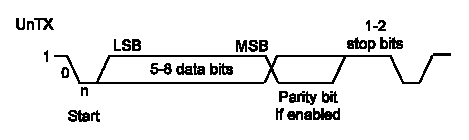
\includegraphics[width=0.5\textwidth] {figuras/uartTiva.eps}
	\caption{Sinal de Transmissão UART no Tiva TM4C1294NCPDT}
	\label{fig:uartTiva}
\end{figure}


\section{Na TivaWare}



\chapter{Barramento SPI}
A Interface de Periféricos Serial, ou SPI (\emph{Serial Peripheral Interface}) nada mais é do que um dispositivo periférico usado na transmissão e recepção serial de dados. Sendo uma comunicação síncrona, a SPI necessita de uma fonte de clock de referência para se estabelecer, além de um sinal de \emph{chip select}, ou \textbf{CS}, para ativar a recepção de dados no dispositivo receptor. Deste modo esta comunicação requer no minimo três vias de transmissão, sendo que a comunicação em cada barramento é unidirecional.

\section{Padrão da Comunicação}

A comunicação SPI possui a maior taxa de transmissão, ou \emph{baud-rate}, dentre os demais protocolos de comunicação usados em microcontroladores, podendo chegar a até a 66Mpbs em periféricos com o AT45BD0100D da Adesto. O que possibilita um  \emph{baud-rate} tão elevado é o fato de que nesta comunicação a recepção e a transmissão de dados é feita separadamente e de forma direta, sem a necessidade de se transmitir bits de inicio ou termino de transmissão, e ainda de modo que o controle da transmissão é realizado pelo sinal CS (Chip Select) e pelo sinal  CLK (Clock).  A figura \ref{fig:SPI} apresenta o padrão de uma comunicação SPI.

\begin{figure}[H]
	\centering
	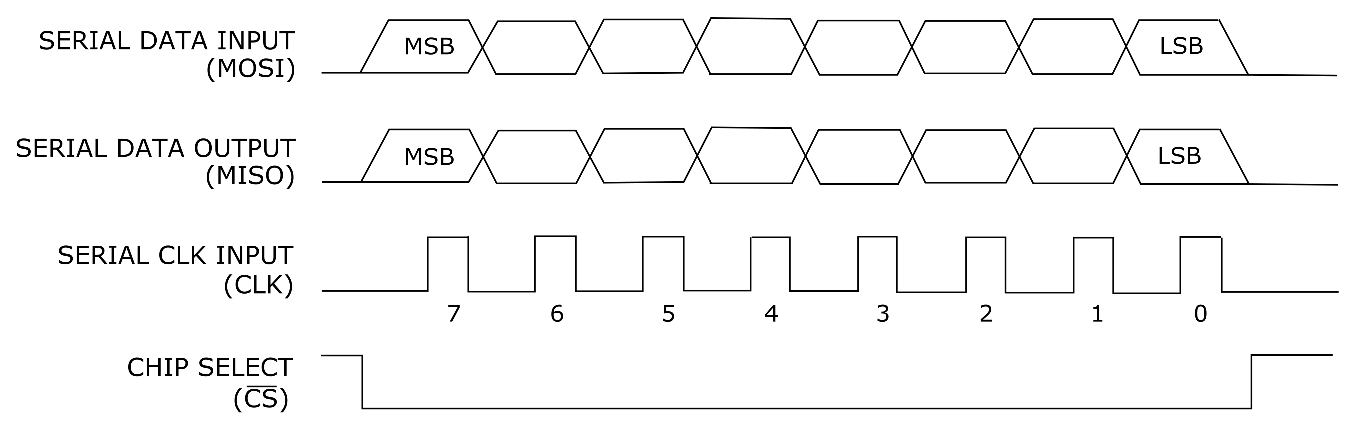
\includegraphics[width=1\textwidth] {figuras/PadraoSPI.eps}
	\caption{Padrão de Comunicação SPI}
	\label{fig:SPI}
\end{figure}

Para transmitir um dado de um dispositivo \textbf{Mestre} para um \textbf{Escravo} é necessário que o \textbf{Mestre} ative o sinal de CS do \textbf{Escravo} e fornecer a ele o sinal de clock de referência. Em seguida bit a bit deve ser transmitido pela porta MOSI \emph{Master Output - Slave Input} de ambos os dispositivos. 

Quando for necessário transmitir um dado de um  \textbf{Escravo} para um \textbf{Mestre}, novamente o \textbf{Mestre} deve ativar o sinal de CS do  \textbf{Escravo} e fornecer a ele o sinal de clock de referência, porém o dado será transmitido bit a bit pela porta MISO \emph{Master Input - Slave Output}. 

\begin{figure}[H]
	\centering
	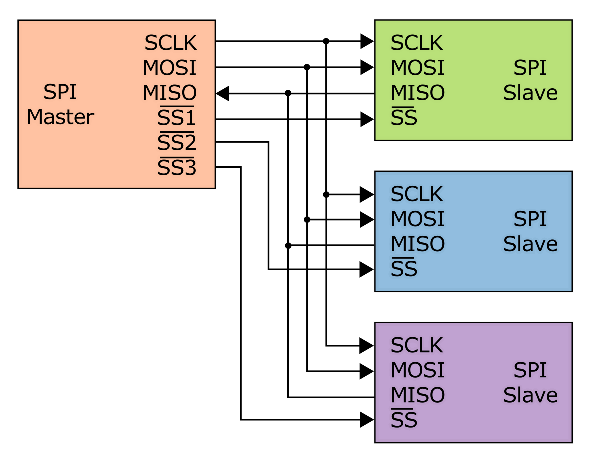
\includegraphics[width=0.6\textwidth] {figuras/BarramentoSPI.eps}
	\caption{Diagrama de Comunicação SPI - Vários Escravos}
	\label{fig:SPIDiagrama}
\end{figure}

A figura  \ref{fig:SPIDiagrama} apresenta um diagrama básico de uma comunicação entre \textbf{Mestre} e vários \textbf{Escravos} através dos de barramentos de dados e de clock em comum.  

\section{SPI do TM4C1294NCPDT}

No Tiva - TM4C1294NCPDT a comunicação SPI se dá através do Interface Serial Quad Sincrona (\emph{Quad Synchronous Serial Interface}), ou QSSI. Há 4 módulos QSSI no Tiva, todos capazes de transmitir dados no modo Advanced, Bi-SSI e Quad-SSI.

No modo de transmissão Bi-SSI, dois pinos de dados são ativados para receber ou transmitir; SSInXDAT0 e o SSInXDAT1. Já no modo de transmissão Quad-SSI, quatro pinos são ativados para receber ou transmitir dados; SSInXDAT0, SSInXDAT1, SSInXDAT2 e SSInXDAT4. 

No modo de transmissão Advanced, a transmissão se realiza de modo que ao transmitir um dado por um pino, o outro pino fica impossibilitado de receber, e vice-versa.

A forma de transmissão dos módulos QSSI podem ser alterados entre os formatos \emph{Texas Instruments synchronous serial} e \emph{Freescale SPI}. Logo para transmitir em modo SPI basta somente selecionar o modo \emph{Freescale SPI}, podendo utilizar tanto o modo de transmissão Bi- ou  Quad-SSI.

No modo de comunicação SPI, tem-se um \emph{baud rate} máximo de 2MHz e uma FIFO para transmissão e outra para recepção ambas com capacidade de 16x8 bits. É possível alternar a fonte de clock de referência da transmissão entre o clock padrão do sistema (SYSCLK) e o clock alternativo (ALTCLK), contando ainda com um divisor de clock de 8 bits, que possibilita dividir o clock de 1 até 254 vezes.  

Como é comum na comunicação SPI o Tiva possui portas para transmissão, recepção e clock exclusiva para cada  módulo de comunicação. A tabela \ref{tab:CanaisSPI} apresenta as referidas portas para comunicação SPI.

\begin{table}[H]
	\centering
	\caption{Canais do SPI - Tiva TM4C1294NCPDT \cite{DATASHEET_TIVA} }
	\label{tab:CanaisSPI}
	\begin{tabular}{|c|c|c|c|l|}
		\rowcolor[HTML]{000000} 
		{\color[HTML]{FFFFFF} Pino}  & {\color[HTML]{FFFFFF} Mux/Função} & {\color[HTML]{FFFFFF} Tipo} & {\color[HTML]{FFFFFF} Buffer} & {\color[HTML]{FFFFFF} Descrição}  \\
		\hline
		SSI0CLK   & PA2 (15) & I/O & TTL & SPI Módulo 0, sinal de clock   \\
		\hline
		SSI0XDAT0 & PA4 (15) & I/O & TTL & SPI Módulo 0, MISO \\
		\hline
		SSI0XDAT1 & PA5 (15) & I/O & TTL & SPI Módulo 0, MOSI \\
		\hline
		SSI1CLK   & PB5 (15) & I/O & TTL & SPI Módulo 1, sinal de clock   \\
		\hline
		SSI1XDAT0 & PE4 (15) & I/O & TTL & SPI Módulo 1, MISO  \\
		\hline
		SSI1XDAT1 & PE5 (15) & I/O & TTL & SPI Módulo 1, MOSI  \\
		\hline
		SSI2CLK   & PB5 (15) & I/O & TTL & SPI Módulo 2, sinal de clock   \\
		\hline
		SSI2XDAT0 & PD1 (15) & I/O & TTL & SPI Módulo 2, MISO  \\
		\hline
		SSI2XDAT1 & PD0 (15) & I/O & TTL & SPI Módulo 2, MOSI  \\
		\hline
		SSI3CLK   & PQ0 (14) & I/O & TTL & SPI Módulo 3, sinal de clock   \\
		          & PF3 (14) &     &     &                                \\
		\hline
		SSI3XDAT0 & PQ2 (14) & I/O & TTL & SPI Módulo 3, MISO  \\
		          & PF1 (14) &     &     &                     \\
		\hline
		SSI3XDAT1 & PQ3 (14) & I/O & TTL & SPI Módulo 3, MOSI  \\
		          & PF0 (14) &     &     &                     \\
		\hline
	\end{tabular}
\end{table}


\section{SPI Na TivaWare}

\section{Exemplo}

\chapter{Conversor Analógico/Digital ADC}
O ADC (\emph{Analog-To-Digital Converter}) é um periférico responsável por realizar a conversão de uma grandeza analógica de tensão para um valor correspondente digital. Para realizar esta conversão pode-se implementar vários  tipos circuito, como o conversor flash, ou o conversor de aproximações sucessivas, ou ainda conversor integrador simples ou de rampa dupla. Porém o  circuito de conversão mais usado em circuito integrados atualmente é o conversor de aproximações sucessivas, o qual também usado como AD no Tiva TM4C1294NCPDT. 


\section{ADC de Aproximações Sucessivas}

\begin{figure}[H]
	\centering
	\fbox{
	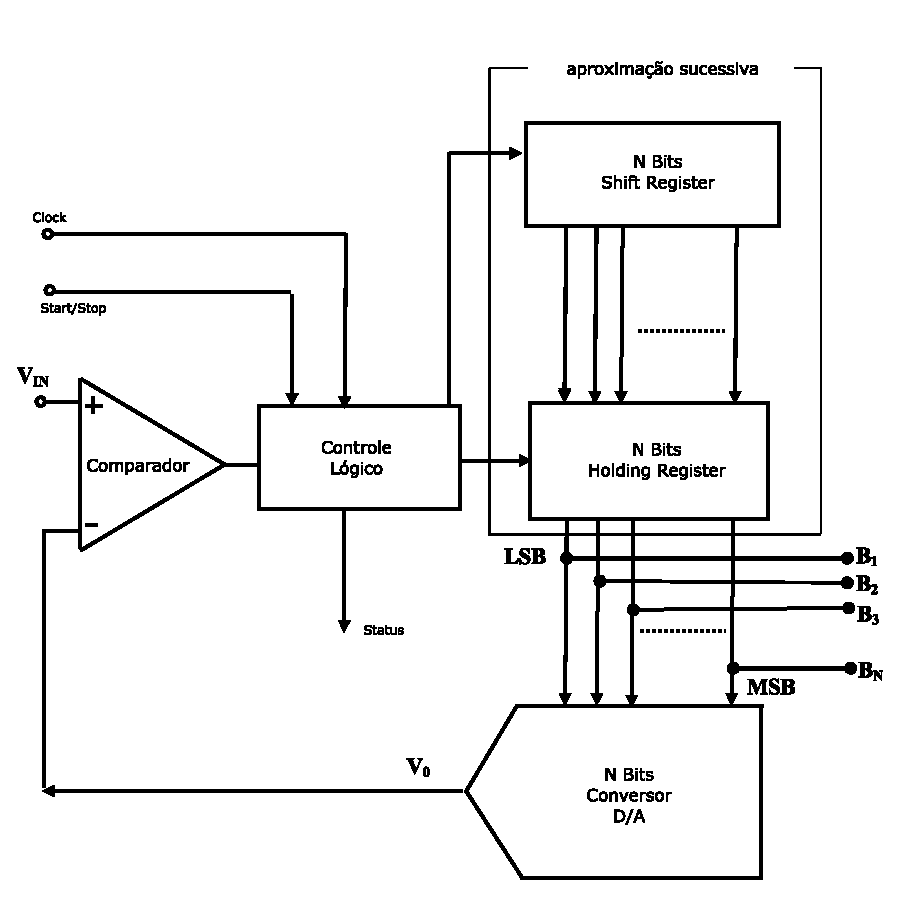
\includegraphics[width=0.5\textwidth] {figuras/ConversorAD.eps}}
	\caption{Conversor A/D tipo Aproximação Sucessiva}
	\label{fig:ConversorAD}
\end{figure}

 A figura \ref{fig:ConversorAD} apresenta o diagrama básico de funcionamento de um conversor de aproximações sucessivas. Nota-se que tal conversor utiliza a técnica de realimentação para relacionar uma voltagem analógica de entrada com um código digital, através de um conversor DA (\emph{Digital-To-Analog Converter}) e um comparador. O processo de conversão inicia quando o \emph{Shift Register} e o \emph{Holding Register} são zerados, e então o MSB (\emph{Most Significant Bit}) do \emph{Holding Register} vai para nível alto. Em seguida o comparador relaciona a saída do conversor DA com a tensão $V_{IN}$. Se $V_{O} < V_{IN}$ a conversão chega ao fim, porém se isso não for verdade a etapa se repete e MSB vai para nível baixo e o segundo SB vai para nível alto. E assim se dá a conversão. 

\section{ADC do TM4C1294NCPDT}

O Tiva TM4C1294NCPDT possui 2 módulos de conversão AD  de 12-bit, que podem ser usados em qualquer um das 20 entradas de sinal analógico. É possível realizar amostragens sequenciais entre os canais ou no mesmo canal repetidamente com intervalos de tempo  programáveis. Cada módulo AD possui 8 comparadores que possibilitam realizar comparações entre os sinais de entrada e  valores pré-definidos, para que assim possa ser realizado as mais diversas operações.  Ainda é possível usar um \emph{trigger} diferente para cada um dos módulos, ou usar um \emph{trigger} para acionar ambos os módulos.

A tabela \ref{tab:CanaisADC} apresenta os pinos de entrada para os módulos ADC0 e ADC1, com a descrição do nome do pino de entrada, o numero referente a este pino, sua função e o tipo de \emph{buffer} usado. Nesta mesma tabela temos o  pino chamado de $VREFA+$ que é o pino da tensão de referência usado pelo AD. O $VREFA+$ corresponde o valor máximo que o conversor DA, usado pelo AD para realizar a comparação com a tensão de entrada, pode atingir. 

A tensão $VREFA+$ é extremamente importante para se realizar a conversão AD, pois se este valor não for selecionado de forma adequada pode-se acarretar problemas no valor digital. A tensão $VREFA+$ pode ser alternada entre uma fonte de referência interna ou externa. 

\begin{center}
\begin{longtable}{|c|c|c|c|c|c|}
	\rowcolor[HTML]{000000}
	{\color[HTML]{FFFFFF} Pino} & {\color[HTML]{FFFFFF} $n^{o}$} & {\color[HTML]{FFFFFF} Mux/Função} & {\color[HTML]{FFFFFF} Tipo} & {\color[HTML]{FFFFFF} Buffer} & {\color[HTML]{FFFFFF} Descrição}            \\
	AIN0                        & 12                             & PE3                               & I                           & Analógico                     & ADC - Entrada 0                             \\
	\hline
	AIN1                        & 13                             & PE2                               & I                           & Analógico                     & ADC - Entrada 1                             \\
	\hline
	AIN2                        & 14                             & PE1                               & I                           & Analógico                     & ADC - Entrada 2                             \\
	\hline
	AIN3                        & 15                             & PE0                               & I                           & Analógico                     & ADC - Entrada 3                             \\
	\hline
	AIN4                        & 128                            & PD7                               & I                           & Analógico                     & ADC - Entrada 4                             \\
	\hline
	AIN5                        & 127                            & PD6                               & I                           & Analógico                     & ADC - Entrada 5                             \\
	\hline
	AIN6                        & 126                            & PD5                               & I                           & Analógico                     & ADC - Entrada 6                             \\
	\hline
	AIN7                        & 125                            & PD4                               & I                           & Analógico                     & ADC - Entrada 7                             \\
	\hline
	AIN8                        & 124                            & PE5                               & I                           & Analógico                     & ADC - Entrada 8                             \\
	\hline
	AIN9                        & 123                            & PE4                               & I                           & Analógico                     & ADC - Entrada 9                             \\
	\hline
	AIN10                       & 121                            & PB4                               & I                           & Analógico                     & ADC - Entrada 10                            \\
	\hline
	AIN11                       & 120                            & PB5                               & I                           & Analógico                     & ADC - Entrada 11                            \\
	\hline
	AIN12                       & 4                              & PD3                               & I                           & Analógico                     & ADC - Entrada 12                            \\
	\hline
	AIN13                       & 3                              & PD2                               & I                           & Analógico                     & ADC - Entrada 13                            \\
	\hline
	AIN14                       & 2                              & PD1                               & I                           & Analógico                     & ADC - Entrada 14                            \\
	\hline
	AIN15                       & 1                              & PD0                               & I                           & Analógico                     & ADC - Entrada 15                            \\
	\hline
	AIN16                       & 18                             & PK0                               & I                           & Analógico                     & ADC - Entrada 16                            \\
	\hline
	AIN17                       & 19                             & PK1                               & I                           & Analógico                     & ADC - Entrada 17                            \\
	\hline
	AIN18                       & 20                             & PK2                               & I                           & Analógico                     & ADC - Entrada 18                            \\
	\hline
	AIN19                       & 21                             & PK3                               & I                           & Analógico                     & ADC - Entrada 19                            \\
	\hline
	&                                &                                   &                             &                               & A tensão de referência                      \\
	&                                &                                   &                             &                               & \multicolumn{1}{l|}{é usada pelo AD para}    \\
	&                                &                                   &                             &                               & \multicolumn{1}{l|}{fixar o valor máximo de} \\
	\multirow{-4}{*}{VREFA+}    & \multirow{-4}{*}{9}            & \multirow{-4}{*}{fixo}            & \multirow{-4}{*}{-}         & \multirow{-4}{*}{Analógico}   & \multicolumn{1}{l|}{conversão.}  \\ 
	\hline
	\caption{Canais de Entrada ADC - Tiva TM4C1294NCPDT \cite{DATASHEET_TIVA} }
	\label{tab:CanaisADC}
\end{longtable}
\end{center}

\section{Na TivaWare}

As principais funções, da biblioteca TivaWare, responsáveis pela configuração e utilização do ADC, são listadas a seguir.

\begin{lstlisting}[style=funcao]
	void ADCSequenceConfigure(uint32_t ui32Base,
							  uint32_t ui32SequenceNum,
							  uint32_t ui32Trigger,
							  uint32_t ui32Priority)
\end{lstlisting}

Configurações básicas do ADC especificado.

\begin{description}
	\item [\ttbu{ui32Base}]\hfill \\
	Base do ADC a ser configurado. Normalmente \textbf{ADC\emph{k}\_BASE}, onde \textbf{\emph{k}} é a letra identificadora do periférico.
	
	\item [\ttbu{ui32SequenceNum}]\hfill \\
	Número da sequência de amostragem.
	
	\item [\ttbu{ui32Trigger}]\hfill \\
	Evento que aciona o amostrador. Definido no formato \textbf{ADC\_TRIGGER\_\emph{k}}, onde \textbf{\emph{k}} pode assumir um dos valores:
	\begin{itemize}
		\item \textbf{PROCESSOR} amostragem iniciada por comando de software.
		\item \textbf{COMP0} amostragem iniciada pelo comparador 0 do ADC.
		\item \textbf{COMP1} amostragem iniciada pelo comparador 1 do ADC.
		\item \textbf{COMP2} amostragem iniciada pelo comparador 2 do ADC.
		\item \textbf{EXTERNAL} amostragem iniciada por uma GPIO de entrada configurada.
		\item \textbf{TIMER} amostragem iniciada pelo temporizador.
		\item \textbf{PWM0} amostragem iniciada pelo PWM 0.
		\item \textbf{PWM1} amostragem iniciada pelo PWM 1.
		\item \textbf{PWM2} amostragem iniciada pelo PWM 2.
		\item \textbf{PWM3} amostragem iniciada pelo PWM 3.
		\item \textbf{ALWAYS} amostragem iniciada repetida e continuamente
	\end{itemize}
\end{description}

\begin{lstlisting}[style=funcao]
	void ADCSequenceStepConfigure(uint32_t ui32Base,
								  uint32_t ui32SequenceNum,
								  uint32_t ui32Step,
								  uint32_t ui32Config)
\end{lstlisting}

Configura o intervalo de amostragem do ADC especificado.

\begin{description}
	\item [\ttbu{ui32Base}]\hfill \\
	Base do ADC a ser configurado. Normalmente \textbf{ADC\emph{k}\_BASE}, onde \textbf{\emph{k}} é a letra identificadora do periférico.
	
	\item [\ttbu{ui32SequenceNum}]\hfill \\
	Número da sequência de amostragem.
	
	\item [\ttbu{ui32Step}]\hfill \\
	Intervalo de amostragem do ADC.
	
	\item [\ttbu{ui32Config}]\hfill \\
	Configuração da amostragem. Pacote de OU lógico de valores no formato \textbf{ADC\_CTL\_\emph{k}}, onde \textbf{\emph{k}} pode assumir os valores:
	\begin{itemize}
		\item \textbf{TS} amostragem do sensor de temperatura interno.
		\item \textbf{IE} amostragem gera interrupção.
		\item \textbf{END} amostragem por sequencia e seleção.
		\item \textbf{D} amostragem por seleção diferencial.
		\item \textbf{CH\emph{k}} seleciona canal de entrada como canal \textbf{\emph{k}}, onde \textbf{\emph{k}} assume valores de 0 a 23.
		\item \textbf{CMP\emph{k}} seleciona comparador \textbf{\emph{k}} para ser utilizado, onde \textbf{\emph{k}} assume valores de 0 a 7.
	\end{itemize}
\end{description}

\begin{lstlisting}[style=funcao]
	void ADCSequenceEnable(uint32_t ui32Base,
						   uint32_t ui32SequenceNum)
\end{lstlisting}

Habilita a sequência de amostragem.

\begin{description}
	\item [\ttbu{ui32Base}]\hfill \\
	Base do ADC a ser configurado. Normalmente \textbf{ADC\emph{k}\_BASE}, onde \textbf{\emph{k}} é a letra identificadora do periférico.
	
	\item [\ttbu{ui32SequenceNum}]\hfill \\
	Número da sequência de amostragem.
\end{description}

\begin{lstlisting}[style=funcao]
	void ADCSequenceDisable(uint32_t ui32Base,
							uint32_t ui32SequenceNum)
\end{lstlisting}

Desabilita a sequência de amostragem.

\begin{description}
	\item [\ttbu{ui32Base}]\hfill \\
	Base do ADC a ser configurado. Normalmente \textbf{ADC\emph{k}\_BASE}, onde \textbf{\emph{k}} é a letra identificadora do periférico.
	
	\item [\ttbu{ui32SequenceNum}]\hfill \\
	Número da sequência de amostragem.
\end{description}

\begin{lstlisting}[style=funcao]
	int32_t ADCSequenceDataGet(uint32_t ui32Base,
							   uint32_t ui32SequenceNum,
							   uint32_t *pui32Buffer)
\end{lstlisting}

Pega o valor gerado na amostragem.

\begin{description}
	\item [\ttbu{ui32Base}]\hfill \\
	Base do ADC a ser lido. Normalmente \textbf{ADC\emph{k}\_BASE}, onde \textbf{\emph{k}} é a letra identificadora do periférico.
	
	\item [\ttbu{ui32SequenceNum}]\hfill \\
	Número da sequência de amostragem.
	
	\item [\ttbu{pui32Buffer}]\hfill \\
	Ponteiro para uma região de memória alocada. Onde será armazenado o valor lido.
\end{description}

\begin{lstlisting}[style=funcao]
	int32_t ADCSequenceDataGet(uint32_t ui32Base,
							   uint32_t ui32SequenceNum,
							   uint32_t *pui32Buffer)
\end{lstlisting}

Pega o valor gerado na amostragem.

\begin{description}
	\item [\ttbu{ui32Base}]\hfill \\
	Base do ADC a ser lido. Normalmente \textbf{ADC\emph{k}\_BASE}, onde \textbf{\emph{k}} é a letra identificadora do periférico.
	
	\item [\ttbu{ui32SequenceNum}]\hfill \\
	Número da sequência de amostragem.
	
	\item [\ttbu{pui32Buffer}]\hfill \\
	Ponteiro para uma região de memória alocada. Onde será armazenado o valor lido.
\end{description}

\begin{lstlisting}[style=funcao]
	int32_t ADCSequenceOverflow(uint32_t ui32Base,
								uint32_t ui32SequenceNum)
\end{lstlisting}

Informa se houve uma perda de leitura, antes de ter lido o valor antigo ocorreu uma nova amostragem.

\begin{description}
	\item [\ttbu{ui32Base}]\hfill \\
	Base do ADC a ser lido. Normalmente \textbf{ADC\emph{k}\_BASE}, onde \textbf{\emph{k}} é a letra identificadora do periférico.
	
	\item [\ttbu{ui32SequenceNum}]\hfill \\
	Número da sequência de amostragem.
\end{description}

\begin{lstlisting}[style=funcao]
	void ADCProcessorTrigger(uint32_t ui32Base,
							 uint32_t ui32SequenceNum)
\end{lstlisting}

Causa uma leitura do ADC invocada pelo processador. Gatilho por software.

\begin{description}
	\item [\ttbu{ui32Base}]\hfill \\
	Base do ADC a ser chamado. Normalmente \textbf{ADC\emph{k}\_BASE}, onde \textbf{\emph{k}} é a letra identificadora do periférico.
	
	\item [\ttbu{ui32SequenceNum}]\hfill \\
	Número da sequência de amostragem.
\end{description}

\begin{lstlisting}[style=funcao]
	void ADCIntRegister(uint32_t ui32Base,
						uint32_t ui32SequenceNum,
						void (*pfnHandler)(void))
\end{lstlisting}

Configura rotina de tratamento de interrupção do ADC.

\begin{description}
	\item [\ttbu{ui32Base}]\hfill \\
	Base do ADC a ser configurada. Normalmente \textbf{ADC\emph{k}\_BASE}, onde \textbf{\emph{k}} é a letra identificadora do periférico.
	
	\item [\ttbu{ui32SequenceNum}]\hfill \\
	Número da sequência de amostragem.
	
	\item [\ttbu{pfnIntHandler}]\hfill \\
	Ponteiro da função de tratamento. Esta não deve receber nada como parâmetro e nem retornar nada.
	
\end{description}

\begin{lstlisting}[style=funcao]
	void ADCIntEnable(uint32_t ui32Base,
					  uint32_t ui32SequenceNum)
\end{lstlisting}

Habilita as interrupções do ADC.

\begin{description}
	\item [\ttbu{ui32Base}]\hfill \\
	Base do ADC a ser configurada. Normalmente \textbf{ADC\emph{k}\_BASE}, onde \textbf{\emph{k}} é a letra identificadora do periférico.
	
	\item [\ttbu{ui32SequenceNum}]\hfill \\
	Número da sequência de amostragem.
\end{description}

\begin{lstlisting}[style=funcao]
	void ADCIntDisable(uint32_t ui32Base,
					   uint32_t ui32SequenceNum)
\end{lstlisting}

Habilita as interrupções do ADC.

\begin{description}
	\item [\ttbu{ui32Base}]\hfill \\
	Base do ADC a ser configurada. Normalmente \textbf{ADC\emph{k}\_BASE}, onde \textbf{\emph{k}} é a letra identificadora do periférico.
	
	\item [\ttbu{ui32SequenceNum}]\hfill \\
	Número da sequência de amostragem.
\end{description}

\begin{lstlisting}[style=funcao]
	void ADCIntClear(uint32_t ui32Base,
					 uint32_t ui32SequenceNum)
\end{lstlisting}

Limpa a \emph{flag} de interrupções do ADC.

\begin{description}
	\item [\ttbu{ui32Base}]\hfill \\
	Base do ADC a ser configurada. Normalmente \textbf{ADC\emph{k}\_BASE}, onde \textbf{\emph{k}} é a letra identificadora do periférico.
	
	\item [\ttbu{ui32SequenceNum}]\hfill \\
	Número da sequência de amostragem.
\end{description}

\section{Exemplo}

A seguir, é apresentado um código de configuração do ADC. Um exemplo mais elaborado é apresentado na Seção \ref{sec:exPwm}.

\begin{lstlisting}[style=citacao]
// Habilita ADC0
MAP_SysCtlPeripheralEnable(SYSCTL_PERIPH_ADC0);
// Aguarda 3 SysCtlDelay. Aproximadamente 10 ciclos de clock
MAP_SysCtlDelay(3);

// Desabilitar Interrupcao do ADC para configura-la
MAP_IntDisable(INT_ADC0SS0);
MAP_ADCIntDisable(ADC0_BASE, 0);
MAP_ADCSequenceDisable(ADC0_BASE, 0);

//Configurando ADC
MAP_ADCHardwareOversampleConfigure(ADC0_BASE, 4);
MAP_ADCSequenceConfigure(ADC0_BASE, 0,
	ADC_TRIGGER_PROCESSOR, 0);
MAP_ADCSequenceStepConfigure(ADC0_BASE, 0, 0,
	ADC_CTL_IE | ADC_CTL_END | ADC_CTL_CH0);
MAP_ADCSequenceEnable(ADC0_BASE, 0);

// Habilitando Interrupcao do ADC
MAP_ADCIntClear(ADC0_BASE, 0);
MAP_ADCIntEnable(ADC0_BASE, 0);
MAP_IntEnable(INT_ADC0SS0);
\end{lstlisting}


\chapter{Modulação por largura de Pulso (PWM)}

PWM (Pulse Width Modulation) é um modulação baseada na conversão linear de um valor em escala de tensão para outro em escala de \emph{Duty Cicle} aplicado a uma onda quadrada de amplitude qualquer. Este tipo de modulação é utilizada em diversas aplicações eletrônicas. 

\section{Modos de Funcionamento}

Para criar uma modulação PWM é necessário criar uma onda periódica linear e variante no tempo, que se consiga comparar com o sinal que se deseja converter em PWM. Logo o tipo de onda necessária neste modulação é a onda triangular ou a onda dente de serra. Para melhor compreensão a onda triangular ou dente de serra será denominada aqui de onda portadora, e o sinal ao qual se deseja converter em PWM será denominado sinal modulante.
  
Para a implementação digital deste método pode ser feito através uma comparação direta entre os módulos dos dois sinais. Quando o modulo do sinal modulante for maior do que o  módulo da portadora  o sinal modulado vai para nível alto. Porém quando o módulo do sinal modulante for menor do que o módulo da portadora o sinal  modulado vai para zero. A grande diferença da implementação digital é que o sinal da portadora é gerado internamente através de um contador, que pode trabalhar no modo de contagem \emph{Down}, \emph{Up} ou \emph{UpDown}.

Quando o sinal da portadora é gerado através de um contador \emph{Down} ou \emph{Up}  a frequência do sinal modulado será igual a frequência do contador dividido pelo numero máximo de contagens. Já quando o sinal da portadora é gerador por um contador\emph{UpDown} a frequência do sinal modulado será igual a frequência do contador dividido por duas vezes o numero máximo de contagens. Sendo que o numero máximo de contagens deve ser maior ou igual ao modulo do sinal modulante. A Figura \ref{fig:Down} e a Figura \ref{fig:UpDown} apresentam melhor o modo como a geração de PWM é realizada digitalmente.  

\begin{figure}[H]
	\centering
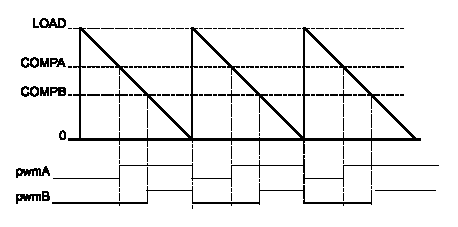
\includegraphics[width=0.8\textwidth] {figuras/Down.eps}
	\caption{PWM modo Down \cite{DATASHEET_TIVA}}
	\label{fig:Down}
\end{figure}

\begin{figure}[H]
	\centering
	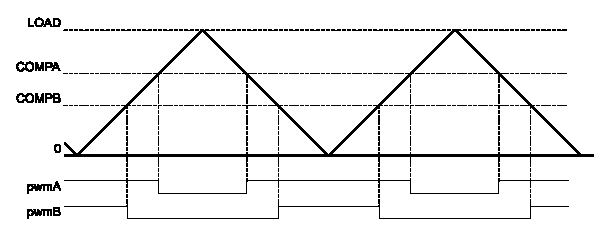
\includegraphics[width=0.8\textwidth] {figuras/UpDown.eps}
	\caption{PWM modo Down \cite{DATASHEET_TIVA}}
	\label{fig:UpDown}
\end{figure}

Tanto na Figura \ref{fig:Down} quanto na Figura \ref{fig:UpDown} os valores de \emph{LOAD}, \emph{COMPA}, \emph{COMPB}, \emph{pwmA} e \emph{pwmB} são referentes aos registradores presente do Tiva - TM4C1294NCPD, responsáveis pela modulação PWM. Tais registradores serão melhor abordados na próxima seção.  

\section{PWM do TM4C1294NCPDT}

O Tiva - TM4C1294NCPD possui um módulo PWM com quatro blocos geradores e seus respectivos blocos de controle, disponibilizando oito saídas PWM.  Através dos blocos de controle é possível escolher qual a polaridade de cada sinal PWM, e o seu respectivo pino. Cada bloco gerador produz 2 sinais PWM com a mesma frequência, porém ambos podem ter \emph{Duty Cicle} independentes ou \emph{Duty Cicle} complementares, com uma intervalo de \emph{Dead Band}. 

Como a maioria das aplicações com PWM é destinada ao chaveamento, o Tiva - TM4C1294NCPD possui não só uma configuração de geração PWM complementar com \emph{Dead Band}, recurso essencial para acionamento de pontes H, como também possui 4 pinos de entrada para um sistema de controle de falha, um para cada gerador PWM.

Para gerar a onda portadora o Tiva possui um contador de 16 bits capaz de realizar contagens no modo \emph{Down} e \emph{UpDown}, sendo possível atualizar o valor da contagem máxima (\emph{LOAD}). Cada um dos geradores PWM possuem ainda dois comparadores distintos (\emph{COMPA} e \emph{COMPB}), responsáveis por gerar os sinais PWM e que podem ser usados para gerar interrupções. 

Quando um comparador está configurado para provocar interrupções esta ocorre toda vez que o valor do comparador selecionado for maior do que o valor de \emph{LOAD}.  A Figura \ref{fig:PWMCountDownMode} demonstra o modo como as os sinais de interrupção são provocados pelos comparadores no modo \emph{Down}, e a Figura \ref{fig:PWMCountUpDownMode} demonstra o mesmo no modo \emph{UpDown}.

\begin{figure}[H]
	\centering
	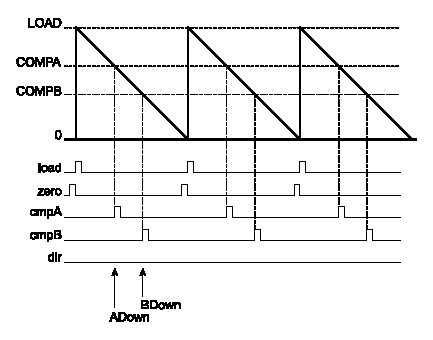
\includegraphics[width=0.8\textwidth] {figuras/PWMCountDownMode.eps}
	\caption{PWM modo Down \cite{DATASHEET_TIVA}}
	\label{fig:PWMCountDownMode}
\end{figure}

\begin{figure}[H]
	\centering
	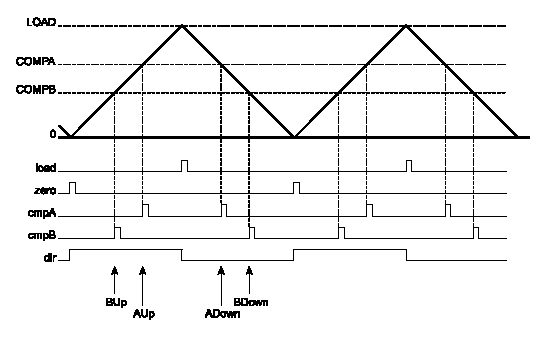
\includegraphics[width=0.8\textwidth] {figuras/PWMCountUpDownMode.eps}
	\caption{PWM modo Down \cite{DATASHEET_TIVA}}
	\label{fig:PWMCountUpDownMode}
\end{figure}

A tabela \ref{tab:CanaisPWM} apresenta os 8 pinos do módulo PWM, sendo estes pinos de saída dos sinais de PWM.  

\begin{center}
	\begin{longtable}{|c|c|c|c|c|}
		\rowcolor[HTML]{000000}
		{\color[HTML]{FFFFFF} Pino} & {\color[HTML]{FFFFFF} $n^{o}$} & {\color[HTML]{FFFFFF} Mux/Função} & {\color[HTML]{FFFFFF} Tipo} & {\color[HTML]{FFFFFF} Descrição}            \\
		M0PWM0    & 42  & PF0 (6) & O & Saída PWM 0\\
		M0PWM1    & 43  & PF1 (6) & O & Saída PWM 1\\
		M0PWM2    & 44  & PF2 (6) & O & Saída PWM 2\\
		M0PWM3    & 45  & PF3 (6) & O & Saída PWM 3\\
		M0PWM4    & 49  & PG0 (6) & O & Saída PWM 4\\
		M0PWM5    & 50  & PG1 (6) & O & Saída PWM 5\\
		M0PWM6    & 63  & PK4 (6) & O & Saída PWM 6\\
		M0PWM7    & 62  & PK5 (6) & O & Saída PWM 7\\
		\hline
		\caption{Canais PWM - Tiva TM4C1294NCPDT \cite{DATASHEET_TIVA} }
		\label{tab:CanaisPWM}
	\end{longtable}
\end{center}

\section{PWM do TM4C1294NCPDT}

\section{Exemplo}


\chapter{Temporizador de Propósito Geral}
\section{Modos de Funcionamento}

\section{Temporizador no TM4C1294NCPDT}

\section{Exemplo}

% \setcounter{minitocdepth}{1}

\chapter{Exemplos de aplicação}
Esta seção apresenta alguns exemplos práticos de implementação no TivaWare. É importante ressaltar que esses exemplos foram desenvolvidos para o TM4C1294NCPDT. Sendo assim, podem haver incompatibilidades presentes no carregamento destes códigos para algum outro hardware diferente, mesmo suportado pelo TivaWare.

\section{Listagem de Periféricos pela UART}

O seguinte software, implementa uma comunicação UART na base de UART 0 do microcontrolador. Ao receber bytes, e detectado algum caractere 'p', é imprimido uma lista com os periféricos disponíveis no microcontrolador. Se for algum outro caractere, somente é exibida uma mensagem informativa.

\lstset{language=C,caption={Código de exemplo},label=DescriptiveLabel}
\lstinputlisting{codigo/UARTecho.c}


\bibliographystyle{abbrv}
\bibliography{bibliografia.bib}

\end{document}